% -*- TeX:RNW:UK -*-
\documentclass[10pt]{beamer}
\usetheme{metropolis}
%\useinnertheme{rectangles}
\setbeamercovered{%
still covered={\opaqueness<1->{15}},
again covered={\opaqueness<1->{40}}}

\hypersetup{colorlinks,linkcolor=black,urlcolor=brown,citecolor=brown}

\usepackage{amsmath,amssymb,amsthm}
\usepackage{unicode-math}

\usepackage{amsmath,amssymb,amsthm}
\usepackage{unicode-math}

% We set the Lucida OTF fonts as default
\usepackage{fontspec}
\setmainfont{Lucida Bright OT}
\setsansfont{Lucida Sans OT}
\setmonofont{Lucida Console DK}[Scale=MatchLowercase]

\newfontfamily\webglyphsfont{WebHostingHub-Glyphs}[Scale=0.7]
\newcommand\webglyphs[1]{{\webglyphsfont\symbol{#1}}}
\newcommand\Discussion{\colorbox{white}{\textcolor{black}{\webglyphs{"F134}}}\xspace}
\newcommand\DiscussionI{\colorbox{black}{\textcolor{white}{\webglyphs{"F134}}}\xspace}
\newcommand\DExamples{\colorbox{black}{\textcolor{white}{\webglyphs{"F134} examples?}}}
\newcommand\Reading{\colorbox{black}{\textcolor{white}{\webglyphs{"F0C1}}}\xspace}
\newcommand\ReadingI{\colorbox{white}{\textcolor{black}{\webglyphs{"F0C1}}}\xspace}
\newcommand\Video{\colorbox{white}{\textcolor{black}{\webglyphs{"F03D}}}\xspace}
\newcommand\Attention{\colorbox{black}{\textcolor{orange}{\webglyphs{"F05A}}}\xspace}
\newcommand\HomeWork{\colorbox{white}{\textcolor{black}{\webglyphs{"F5ED}}}\xspace}
\newcommand\HomeWorkI{\colorbox{black}{\textcolor{white}{\webglyphs{"F5ED}}}\xspace}
\newcommand\Advanced{\colorbox{black}{\textcolor{white}{\webglyphs{"F235}}}\xspace}

\newfontfamily\lineabasicfont{linea-basic-10}
\newcommand\basicicons[1]{{\lineabasicfont\symbol{#1}}}
\newcommand\timeforwards{\basicicons{"0079}}
\newcommand\timebackwards{\basicicons{"0064}}

\newfontfamily\lineaweatherfont{linea-weather-10}
\newcommand\weathericons[1]{{\lineaweatherfont\symbol{#1}}}
\newcommand\meteosun{\weathericons{"E038}}
\newcommand\meteosuncloud{\weathericons{"E042}}
\newcommand\meteorain{\weathericons{"E033}}
\newcommand\meteowind{\weathericons{"E054}}

\newfontfamily\uleaffont{Mini Pics Uprooted Leaf}
\newcommand\uleafmpics[1]{{\uleaffont\symbol{#1}}}
\newcommand\lowplants{\uleafmpics{"00CE}}
\newcommand\mediumplant{\uleafmpics{"006A}}
\newcommand\bush{\uleafmpics{"0039}}
\newcommand\smallplant{\uleafmpics{"0030}}
\newcommand\seedling{\uleafmpics{"002F}}
\newcommand\floweringplant{\uleafmpics{"00CA}}

\newfontfamily\utwigfont{Mini Pics Uprooted Twig}
\newcommand\utwigmpics[1]{{\utwigfont\symbol{#1}}}
\newcommand\grassplant{\utwigmpics{"0033}}

\newfontfamily\uinsectfont{Insect Icons}
\newcommand\uinsect[1]{{\uinsectfont\symbol{#1}}}
\newcommand\bug{\uinsect{"006F}}

\usepackage{polyglossia}
\setdefaultlanguage[variant = british, ordinalmonthday = false]{english}

\usepackage[style=authoryear-comp,firstinits,sortcites,maxcitenames=2,%
    mincitenames=1,maxbibnames=10,minbibnames=10,uniquename=mininit,%
    uniquelist=minyear,sortfirstinits=true]{biblatex}
\addbibresource{../references/ecophys.bib}
\renewcommand{\bibfont}{\small}

\usepackage{abbrev}



\usepackage{tikz}
\usetikzlibrary{positioning,fit,arrows}

\tikzset{
 a/.style
  = {node distance=4em, text width=3.5em, minimum height=4em},
 b/.style
  = {rectangle, draw, fill=gray!10, node distance=4em, text width=6em,
     text centered, rounded corners, minimum height=4em, thick},
 c/.style
  = {circle, draw, dashed, fill=orange!10, inner sep = 0pt, node distance=5em, thick},
 d/.style
  = {rectangle, draw, dashed, fill=red!10, node distance=4em, text width=6em,
     text centered, rounded corners, minimum height=4em, thick},
 l/.style
  = {draw, -latex, thick},
 lr/.style
  = {draw, latex-latex, thick, red},
 lb/.style
  = {draw, -latex, thick, blue},
  lo/.style
  = {draw, -latex, thick, orange},
  lg/.style
  = {draw, -latex, thick, green},
  mylabel/.style
  ={text width=6.5em, text centered}
}

\newcommand*{\Px}{\ensuremath{\mathrm{P}}\xspace}
\newcommand*{\Pxfr}{\ensuremath{\mathrm{P_{fr}}}\xspace}
\newcommand*{\Pxr}{\ensuremath{\mathrm{P_r}}\xspace}
\newcommand*{\Pxtot}{\ensuremath{\mathrm{P_{tot}}}\xspace}

%\newcommand*{\COtwo}{\ensuremath{\textrm{CO}_2}\xspace}

\newcommand*{\nEff}{{\scriptsize 0}\xspace}
\newcommand*{\pEff}{\ensuremath{+}\xspace}
\newcommand*{\mEff}{\ensuremath{-}\xspace}
\newcommand*{\uEff}{?\xspace}

\newcommand*{\myatop}[2]{\genfrac{}{}{0pt}{3}{#1}{#2}}

\begin{document}

\title{IPS-141\\Sensory and Physiological Ecology of  Plants}
\subtitle{8: Phenology}
\author{Pedro J. Aphalo}
\date{January--February 2022}
\institute[Univ.\ of Helsinki]{M.Sc.\ in Plant Biology, University of Helsinki\\[2ex] \url{http://blogs.helsinki.fi/aphalo/}}


  \begin{frame}
    \maketitle
  \end{frame}

  \begin{frame}[c]
    \begin{center}
      \begin{small}
        \copyright 2006--2022 by Pedro J. Aphalo\\
        University of Helsinki, Finland.\\
        \textcolor{blue}{\url{http://blogs.helsinki.fi/senpep-blog/}}\\[2ex]
      \end{small}

      \begin{footnotesize}
        Sensory and Physiological Ecology of Plants slides by Pedro J. Aphalo are licensed under a Creative Commons Attribution-ShareAlike 4.0 International License.

      
\includegraphics[width=6em]{../figures/copyright/by-sa}\\[2ex]
      \end{footnotesize}
        
        \begin{scriptsize}
        Typeset in Lucida Sans, \textrm{Luicda Bright}, \texttt{Lucida Console} and Lucida Math. Icons from fonts ``WebHostingHub Glyphs'' (under SIL-Open Font License) from \url{https://www.webhostinghub.com/}; ``insect icons'' (free from \url{http://www.woodcutter.es/}); ``linea-basic-10'' and ``linea-weather-10'' (free from \url{https://github.com/linea-io}), ``Mini Pics Uprooted Twig'' and ``Mini Pics Uprooted Twig'' (commercial, from Image Club Graphics, Inc.). Plant icon as .svg by Abdul Wahhab (free from \url{NounProject.com}).

        Illustrations and text quoted from copyrighted sources is excluded from this license and their use should respect the original licenses.
        \end{scriptsize}
    \end{center}
  \end{frame}


  \begin{frame}
    \frametitle{Outline}
    \tableofcontents
  \end{frame}

\section{Phenology}

\begin{frame}{Introduction}
    \begin{itemize}
        \item The study of the timing of biological events of
        the life history of plants and animals, and how
        this timing is controlled by the environment.
        \item According to the seasons of the year, not the daily
        rhythms.
        \item Important both for annual, biennial and perennial
        plants.
        \item Perennial plants: 1) initiation of growth
        (budburst, flowering); 2) growth cessation; 3) leaf senescence; 4) frost hardening and
        dehardening.
        \item[+] See \autocite{Larcher2003} for details, and
        information on species from other latitudes.
    \end{itemize}
\end{frame}

\begin{frame}{Yearly variation}
    \begin{itemize}
        \item Phenological events define the limits of
        phenophases.%
        \item The timing of phenological events will vary from
        year to year depending on the prevailing weather.%
        \item The study of phenology is an ancient science. More
        than a 1000 years ago there were phenological calendars in
        China.%
        \item The basis has been the collection of long time
        series of observations and relating them to weather records.%
        \item More recently an experimental approach has also
        been used.%
    \end{itemize}
\end{frame}

\begin{frame}{The available signals}
    \begin{itemize}
        \item Temperature
        \begin{itemize}
            \item Cold $\rightarrow$ means winter.
            \item Warm $\rightarrow$ means summer.
            \item Stimulus is accumulated: temperature sums related to responses.
        \end{itemize}
        \item Photoperiod (day length)
        \begin{itemize}
            \item Short days $\rightarrow$ means autumn.
            \item Long days $\rightarrow$ means spring.
        \end{itemize}
    \end{itemize}
\end{frame}

\begin{frame}{Daylength and latitude}
    \centering
    \includegraphics[height=0.7\textheight]{figures/Taiz25-16daylength.pdf}\\
    {\small \autocite[from][]{TaiZei2006}}
\end{frame}

\section{Timing of flowering}

\begin{frame}{Flowering at midsummer}
    \centering
    \includegraphics[height=0.7\textheight]{figures/rose}
\end{frame}

\begin{frame}{Flower induction}
    \begin{itemize}
        \item Long-day plants (LDP): \species{Fuchsia}.
        \item Short-day plants (SDP): wheat (not all vars.), \species{Chrysanthemum morifolium}.
        \item Day-neutral plants (DNP): kidney bean (\species{Phaseolus vulgaris}).
        \item Long-short-day plants (LSDP): Kalanchoe, \species{Cestrum nocturnum}.
        \item Short-long-day plants (SLDP): white clover.
    \end{itemize}
\end{frame}

\begin{frame}{LDP vs.\ SDP}
    \begin{description}
        \item[LDP] Plants that flower when the daylength is longer than a given threshold. The day does not need to be particularly long.
        \item[SDP] Plants that flower when the daylength is shorter than a given threshold. The day does not need to be particularly short.
    \end{description}
\end{frame}

\begin{frame}{LDP vs.\ SDP}
    \centering
    \includegraphics[width=\textwidth]{figures/Taiz25-18LDSDflowering.pdf}\\
    {\small \autocite[from][]{TaiZei2006}}
\end{frame}

\begin{frame}{Night length}
    \begin{itemize}
        \item The length of the uninterrupted dark period is what matters.
        \item The night can be ``broken'' by a pulse of light.
    \end{itemize}
\end{frame}

\begin{frame}{Night break}
    \centering
    \includegraphics[width=0.8\textwidth]{figures/Taiz25-19ANightBreak.pdf}\\
    {\small \autocite[from][]{TaiZei2006}}
\end{frame}

\begin{frame}{Night break}
    \centering
    \includegraphics[height=0.7\textheight]{figures/Taiz25-19BNightBreak.pdf}\\
    {\small \autocite[from][]{TaiZei2006}}
\end{frame}

\begin{frame}{Involvement of phytochromes}
    \begin{itemize}
        \item As we saw last week, phytochromes are photoreversible pigments.
        \item They can be mainly in two forms one that absorbs red light and one that absorbs far-red light.
        \item Phytochromes are involved in the sensing of night length.
        \item This can be demonstrated with pulses of red- and far-red light.
    \end{itemize}
\end{frame}

\begin{frame}{Reversion}
    \centering
    \includegraphics[width=0.8\textwidth]{figures/Taiz25-23NightBreaksReversion.pdf}\\
    {\small \autocite[from][]{TaiZei2006}}
\end{frame}


\section{Timing of budburst}

\begin{frame}{Budburst of \emph{Tilia}}
    \begin{centering}
    \includegraphics[height=0.6\textheight]{figures/Bursting_buds.jpg}\\
    \end{centering}
    {\small Jonathan Billinger [CC-BY-SA-2.0 (\url{http://creativecommons.org/licenses/by-sa/2.0})], via Wikimedia Commons.}
\end{frame}

\begin{frame}{Budburst}
    \centering
    \includegraphics[width=0.9\textwidth]{figures/Hari2BudBurstSaarijarvi.pdf}\\
    {\small \autocite[from][]{Hari1991}.}
\end{frame}

\begin{frame}{Models}
    \begin{itemize}
        \item For prediction of phenological events, models can be used.
        \item For prediction of growth of perennial plants, both current
        temperature and the phase of the annual rhythm must the considered.
        \item The phase transitions of the annual rhythm being controlled
        in many cases by temperatures (chilling in some situations) and
        photoperiod (daylength).
    \end{itemize}
\end{frame}

\begin{frame}{Budburst models}
    \centering
    \includegraphics[width=\textwidth]{figures/Hari2BudBurstModels.pdf}\\
    {\small Comparison of prediction of bud burst date as a mean date and by a model that takes into account
    the sum of temperatures above a threshold of 5 C \autocite[from][]{Hari1991}.}
\end{frame}

\begin{frame}{Budburst and chilling}
    \centering
    \includegraphics[height=0.6\textheight]{figures/HanninenDormancyRelease.pdf}\\
    {\small Duration of chilling period (outdoors) and time to bud burst after transfer
    to the indicated temperatures \autocite[from][]{Hanninen1990}.}
\end{frame}

\begin{frame}{Budburst and growth model}
    \centering
    \includegraphics[height=0.7\textheight]{figures/Kanninen1ModelDiagram.pdf}\\
    {\small \autocite[from][]{KanninenEtAl1982}.}
\end{frame}

\begin{frame}{Budburst and growth model}
    \centering
    \includegraphics[width=\textwidth]{figures/Kanninen2Phases.pdf}\\
    {\small \autocite[from][]{KanninenEtAl1982}.}
\end{frame}

\begin{frame}{Budburst and growth model}
    \centering
    \includegraphics[height=0.7\textheight]{figures/Kanninen4Growth.pdf}\\
    {\small \autocite[from][]{KanninenEtAl1982}.}
\end{frame}

\begin{frame}{Elongation growth}
    \centering
    \includegraphics[width=0.75\textwidth]{figures/Lahti8GrowthPine74_75.pdf}\\
    {\small \autocite[from Kanninen 1990 in][]{LahSmo1990}.}
\end{frame}

\begin{frame}{Elongation growth cessation}
    \centering
    \includegraphics[height=0.55\textheight]{figures/Koski4aBetula.pdf}\\
    {\small Stem elongation growth cessation event in silver birch
    seedlings in relation to night length (L) and the temperature
    sum accumulated at the time of the event \autocite[from][]{Koski1985}.}
\end{frame}

\begin{frame}{Elongation growth cessation}
    \centering
    \includegraphics[height=0.55\textheight]{figures/Koski4bPinus.pdf}\\
    {\small Stem elongation growth cessation event in Scots pine
    seedlings in relation to night length (L) and the temperature
    sum accumulated at the time of the event \autocite[from][]{Koski1985}.}
\end{frame}

\begin{frame}{Leaf senescence}
    \fbox{\includegraphics[width=0.23\textwidth]{figures/Birch-1}}%
    \fbox{\includegraphics[width=0.23\textwidth]{figures/Birch-2}}%
    \fbox{\includegraphics[width=0.23\textwidth]{figures/Birch-3}}%
    \fbox{\includegraphics[width=0.23\textwidth]{figures/Birch-4}}\\
    {\small 17, 18, 25, 30 October 2006\\Herttoniemi.\\
    A long photoperiod from the street lamp delays leaf senescence and
    leaf shedding in birch.}
\end{frame}

\section{Cold winters}

\begin{frame}{Growth in trees}
    \centering
    \includegraphics[height=0.7\textheight]{figures/Larcher5-15GrowthInTrees.pdf}\\
    {\small \autocite[from][]{Larcher2003}.}
\end{frame}

\begin{frame}{Annual growth cycle}
    \centering
    \includegraphics[height=0.7\textheight]{figures/Larcher5-16AnnualCycle.pdf}\\
    {\small \autocite[from][]{Larcher2003}.}
\end{frame}

\begin{frame}{Latitudinal `transplant'}
    \centering
    \includegraphics[height=0.7\textheight]{figures/Larcher5-18oldTransplant.pdf}\\
    {\small \autocite[from][]{Larcher1995}.}
\end{frame}

\begin{frame}{Temperature stratification}
    \centering
    \includegraphics[width=\textwidth]{figures/Larcher6-19ColdAirStratification.pdf}\\
    {\small \autocite[from][]{Larcher2003}.}
\end{frame}

\begin{frame}{Frost survival}
    \centering
    \includegraphics[width=0.8\textwidth]{figures/Larcher6-33FrostSurvival.pdf}\\
    {\small \autocite[from][]{Larcher2003}.}
\end{frame}

\begin{frame}{Frost resistance}
    \includegraphics[height=0.7\textheight]{figures/Larcher6-38ColdTolerance.pdf}\\
    {\small \autocite[from][]{Larcher2003}.}
\end{frame}

\begin{frame}{Cold damage}
    \centering
    \includegraphics[height=0.7\textheight]{figures/Lambers6DamagevsSugarsPine.pdf}\\
    {\small \autocite[from][]{LambersEtAl1998}.}
\end{frame}

\begin{frame}{Raunkiaer classification}
    \centering
    \includegraphics[height=0.7\textheight]{figures/Larcher6-40Raunkiaer.pdf}\\
    {\small \autocite[from][]{Larcher2003}.}
\end{frame}

%\begin{frame}{Albedo of vegetation}
%%    \vspace{-0.04\textheight}
%    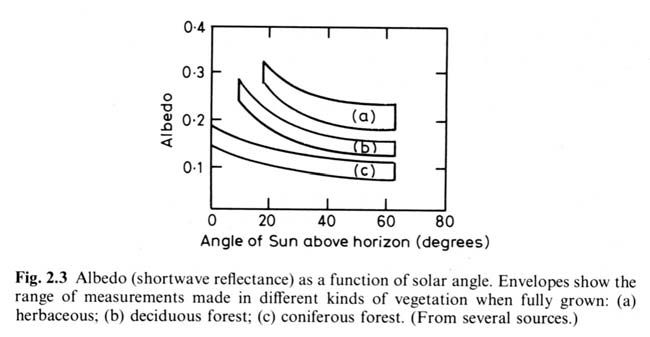
\includegraphics[width=\textwidth]{figures/Grace2.3Albedo.pdf}\\
%    \vspace{-0.01\textheight}
%    {\small \autocite[from][]{Grace1983}.}
%\end{frame}

%\begin{frame}{}
%    \vspace{-0.04\textheight}
%    \includegraphics[height=0.7\textheight]{figures/Willmer.pdf}\\
%    \vspace{-0.01\textheight}
%    {\small \autocite[from][]{WilFri1996}.}
%\end{frame}

%\begin{frame}{}
%    \vspace{-0.04\textheight}
%    \includegraphics[height=0.7\textheight]{figures/Taiz9-2CosineLaw.pdf}\\
%    \vspace{-0.01\textheight}
%    {\small .}
%\end{frame}

%\begin{frame}{Cosine law}
%    \vspace{-0.07\textheight}
%    \twocolumn[lcolwidth=0.57\linewidth,rcolwidth=0.37\linewidth]{
%    \includegraphics[height=0.8\textheight]{figures/Taiz9-2CosineLaw.pdf}}{%
%    \raggedright
%    \vspace{0.1\textheight}
%    {\small Irradiance on a surface depends on the angle of incidence
%    \autocite[from][]{TaiZei2006}.}}
%\end{frame}

  \section*{References}
  \begin{frame}[t,allowframebreaks]
    \frametitle{References}
    \printbibliography
  \end{frame}

\end{document}


